\documentclass[a4paper,12pt]{report}
\usepackage{fontenc}
\usepackage[utf8]{inputenc}
\usepackage[english]{babel}
\usepackage[pdftex]{graphicx} 
\usepackage{listings}
%\setcounter{secnumdepth}{5}
%\setcounter{tocdepth}{3}
\graphicspath {{figures/}}

\textwidth 6.3 in % Width of text line.
    \textheight 9.2 in
    \oddsidemargin 0 in      %   Left margin on odd-numbered pages.
    \evensidemargin 0 in      %   Left margin on even-numbered pages.
    \topmargin 0.2 in
    \headheight 0 in       %   Width of marginal notes.
    \headsep 0 in
    \topskip 0 in

\title{DRescue - Natural Disaster Alert and Rescue}
\author{Samantha Bandini\\Elisa Casadio\\Martina Giovanelli\\Anna Giulia Leoni\\Sofia Rosetti}
\date{\today}

\begin{document}

\maketitle

\tableofcontents

\chapter{Introduction}

The project consists in a monitoring and rescue system in case of natural disasters. 

There is a smartphone application which allows users to alert in the event of hearth-\\quake, landslide, fire and other emergencies.
Alerts are collected and processed with the aim of informing the civil protection of the area in order to coordinate rescue teams.
Civil protection desktop applications communicate with each other to get information about available or occupied rescue teams.

User side there is a native Android application used to warn a natural disaster, sending an alert containing the position to the server.

Civil protection side there is a desktop application used to coordinate rescues.

Each civil protection manages a single district, but each rescue team can join different civil protections. This is why coordination is important in order to know real-time which teams are available and, if not, when they will be.


\chapter{Software development process}

(modalità di divisione in itinere dei task, meeting/interazioni pianificate, modalità di revisione in itinere dei task, scelta degli strumenti di test/build/continuous integration)\\
%•	uno studente (ad esempio, chi ha l'idea del progetto) fungerà da product owner, oltre che da sviluppatore\\
%•	in un meeting iniziale si rediga un product backlog, e si definisca un primo sprint organizzativo (preparazione della build, identificazione requisiti base e architettura)\\
%•	si definiscano via-via delle sprint da 25-30 ore di lavoro (una settimana full-time), in modo da realizzarne 3-4 in tutto\\
%•	si cerchi ad ogni sprint di ottenere risultati "tangibili", con già un valore per gli stakeholder (i docenti)\\
%•	si tenga anche uno sprint backlog, e si facciano meeting frequenti, e meeting a inizio/fine sprint (con brevissimo report del risultato, anch'esso da tenere in versione)\\

%*) Le scelte tecnologiche non dovrebbero essere anticipate troppo per ovvi motivi.. prima le fate prima impattano tutta la parte successiva e quindi diventano più difficilmente riconsiderabili (comunque in linea di principio ogni scelta potrebbero stare ovunque, dai requirement fino all'implementazione) \\



\section{Development methodology}

%Per lo sviluppo del sistema si è deciso di adottare un processo Agile. Ciò ha comportato una serie di incontri iniziali che sono stati essenziali per fare un setup dei tool e creare un workflow che fosse omogeneo tra tutti i membri del gruppo, per far sì che si posassero le fondamenta per il lavoro dei mesi a venire

%La metodologia Scrum è stata presa e rivisitata, tenendo in considerazione di volta in volta le esigenze e le capacità di comunicazione intrinseche tra i membri del gruppo. Un primo esempio di ciò si è riscontrato ad esempio nell’evitare i "stand-up meeting" giornalieri, optando per dei più opportuni meeting tra membri di sottogruppi via VoIP.
%Per ciò che riguarda gli strumenti di Build è stato fatto un estensivo uso di Gradle, in maniera tale che risultasse più pratico utilizzare anche librerie Java all’interno del sistema.

%Inoltre, si è scelto di utilizzare la libreria ScalaTest come strumento per svolgere i test. Essi ricoprono quasi totalmente la parte di model e di controller del codice Client e possono essere visionati nel package src/test. Invece, per quanto concerne il sistema ad attori, presente sia nel codice Client che in quello Server, non vi sono test ma, si è comunque verificata la corretta interazione tra le parti simulando lo scambio di messaggi tra di esse e verificando, in ultimo, l’esattezza del contenuto del messaggio ricevuto



For managing product develop we were inspired by Scrum framework, an iterative and incremental agile software development methodology.
According to Scrum method we decided to have face-to-face meeting as often as possible and when not possible due to personal commitments we planned meeting via VoIP. \\
We have chosen Sofia Rosetti as Product Owner but we proceeded working together and giving always advices and ideas each others.

Despite commitments we tried to organize face-to-face meetings at least once every two weeks, most frequently in the first and last period. So, working at home, we tried to follow the following meeting mode: \\
Every morning teams member available to work on that day had a morning meeting (few minutes) via VoIP or, most frequently, via instant chat, to plan the daily job.\\
Often, in addition to that concise morning meeting, we made a brief evening meeting to aware others members about problems encountered or doubts during work.

We planned Sprint meeting (in addition to the specified daily meetings) as follows:\\
Before each sprint, a sprint planning was organized (max one hour) in which all group members were present. At the end of each sprint, we all met together again to do sprint reviews and sprint retrospectives. Except for the first sprint, these two operations took place on the same day.\\
During the Sprint Review meeting one member at time presented to the others in a few minutes what was done, even with brief examples.

Unfortunately, due to external commitments or personal reasons every member couldn't dedicate only to this single project, for this reasons, we couldn't even split equally the tasks between members for every sprint or split every sprints with equal amount of hours. \\ %TODO tradurre sotto
La gestione delle sprint si è svolta quindi in modo flessibile, as we can see in the product backlog that could be found together with the release %TODO tradurre bene

Abbiamo cercato di mantenere un product backlog che si evolveva nel corso del tempo, come stima si è scelto di utilizzare le ore di lavoro ( %TODO %TODO
SCRIVERE ULTIMO CAP - ABBIAMO AVUTO PROBLEMI A STIMARE IL LAVORO DELLE VARIE SPRINT E SPESSO CI SIAMO RITROVATE A RIORGANIZZARLE VERSO FINE DELLA SPRINT)\\
Durante la Sprint planning veniva stilata una lista abbastanza generica di Sprint tasks, che veniva poi ridefinita e perfezionata da ognuna di noi nel momento in cui veniva scelta. 


%during the first meeting, we have decided to have weekly meetings where weekly tasks were agreed. During each sprint planning, starting from the product backlog, we reviewed high-priority items and discussed goals in order to define the backlog for the given sprint. Tasks were equally split between team members, in such a way that each member could develop different project features. After every sprint, we discussed what went good and what went bad, talking about them and trying to resolve problems within the following sprint.

%At the beginning we had a sprint planning where all the team decided the goal of a specific sprint. The product backlog table was regularly updated and, at the end of each sprint, we wrote a sprint backlog too. The sprint backlog contains information about a specific sprint, while the product backlog keeps track of each user story that was later deepened by creating many items in Trello, ​a ​​taskboard ​ ​for ​ ​agile ​ ​teams.

%Moreover, ​ ​we ​ ​had ​ ​a ​ ​weekly ​ ​meeting ​ ​to ​ ​sum ​ ​up ​ ​the ​ ​issues ​ ​faced ​ ​during ​ ​the ​ ​development. All the documentation generated by the scrum process was tracked as the entire project:

%Simone app was developed following a standard GitHub workflow: a central repository was created and each member of the team forked a copy into its own repository. After each local feature was finally developed, completed and tested, it was later integrated by creating a pull request. Following this, the central repository contains ​ ​the ​ ​latest ​ ​version ​ ​of ​ ​Simone ​ ​app.

%Agile



%TODO da riguardare
%Each Sprint started with the product backlog (where all the main tasks are defined) followed by the Sprint Backlog where all the created tasks were well discussed and divided in more defined and detailed subtasks. During the first 3-4 Sprints each member of the team used to volunteer to be assigned to one or more tasks. As the development continued, each member was assigned to a well defined and specified sub-system, creating a better organized environment where everybody knew exactly what the other was working on. At the end of each week, we used one hour of our time (Sprint Retrospective) to discuss about what went good and what had to be improved during the next Sprint

\section{Development tools}
Following development support tools have been used:

\begin{itemize}
\item \textbf{IntelliJ IDEA} as integrated software environment
\item \textbf{Java} and \textbf{Scala} as programming languages
\item \textbf{JUnit} and \textbf{ScalaTest} as testing tools
\item \textbf{Git} as version control system
\item \textbf{GitHub} as version control repository
\item \textbf{Gradle} as build automation system
\item \textbf{Travis CI} as continuous integration service
\item \textbf{Trello} as web project management application
\item \textbf{TeamViewer} as team collaboration and working tool
\item \textbf{Google Drive} and \textbf{Dropbox} for sharing files and working simultaneously
\item \textbf{Google Calendar} and \textbf{GTimeReport} for working hours count
\end{itemize}

%TODO Test: JUnit e ScalaTest da specificare nelle singole implementazioni

\chapter{Requirements}
%(2-3 facciate)
%Attenzione ai requirement non funzionali: 1) non siano troppo vaghi altrimenti sono inverificabili, e quindi praticamente inutili; 2) il sistema è distribuito, quindi è inevitable dire cosa vi aspettate in termindi di robustezza a cambiamenti/guasti (quali?, come?), e scalabilità

\section{Functional requirements}

According to agile methodologies in the first sprint we wrote user cases like ``As.. I want.. For..", which have highlighted these functional requirements:

\begin{itemize}
\item \textbf{User side}:
\begin{enumerate}
\item A not logged user has to register or login to access the platform.
\item A user needs to view last fifty alerts of his area, to see what happens nearby.
\item A user needs to send an alert to inform civil protection about a particular event.
\item A user needs to view his profile to check his register information.
\item A user needs to change his password to update it.
\item A user needs to confirm an alert (upvoting it) to increase the alert reliability.
\end{enumerate}
\end{itemize}

\begin{itemize}
\item \textbf{Civil protection side}:
\begin{enumerate}
\item A civil protection has to login to access the platform.
\item A civil protection needs to receive alerts of its area to coordinate the rescues.
\item A civil protection needs to visualize in action rescues to have a general view of rescues and occupied teams.
\item A civil protection needs to enroll a rescue team in to send it when needed.
\item A civil protection needs to receive notifications when a team is occupied in order to know which ones to send.
\item A civil protection needs to decide which team is the most appropriate to send (at discretion of the civil protection user).
\item A civil protection needs to notify the sending of a team for a specific alert in order to intervene in case of emergency.
\item A civil protection needs to notify the end of a rescue to inform other civil protections that the team is available again.
\end{enumerate}
\end{itemize}

\begin{itemize}
\item \textbf{Server side}:
\begin{enumerate}
\item The server has to forward the alerts and the upvotes to the civil protection of the area in order to warn it.
\item The server has to interact with the database as for user and civil protection requests in order to save datas. 
\end{enumerate}
\end{itemize}

\section{Non-functional requirements}
Non-functional requirements have been identified as following:

\begin{itemize}
\item Alerts must have a certain reliability, so that civil protections won't receive untruthful alerts and the database won't be overloaded with too many alerts relative to the same event. This way, users can signal the event easier and faster, query executions are simplified and civil protections can visualize last alerts and alerts with recents upvotes at the top of the list.
\item The mobile application must be user-friendly.
\item Civil protection views must be updated real-time without performing a specific request.
\item Alert information must be saved into a database.
\end{itemize}

\chapter{Architectural design}

The system's components, shown in figure \ref{fig:ArchDesign}, are:

\begin{itemize}
\item a \textbf{mobile application}, whose main purpose is sending alerts to report natural disasters;
\item a \textbf{desktop application}, whose main purpose is monitoring natural disasters and coordinate rescues;
\item a \textbf{remote server}, that communicates with clients to send responses and forward alerts to right civil protections;
\item a \textbf{remote database}, that stores all system data. Only the server can access to the database and retrieve data depending on the requests;
\item \textbf{RabbitMQ}, a message broker that allows communications among clients and between clients and server.
\end{itemize}

\begin{figure}[ht]
\centering
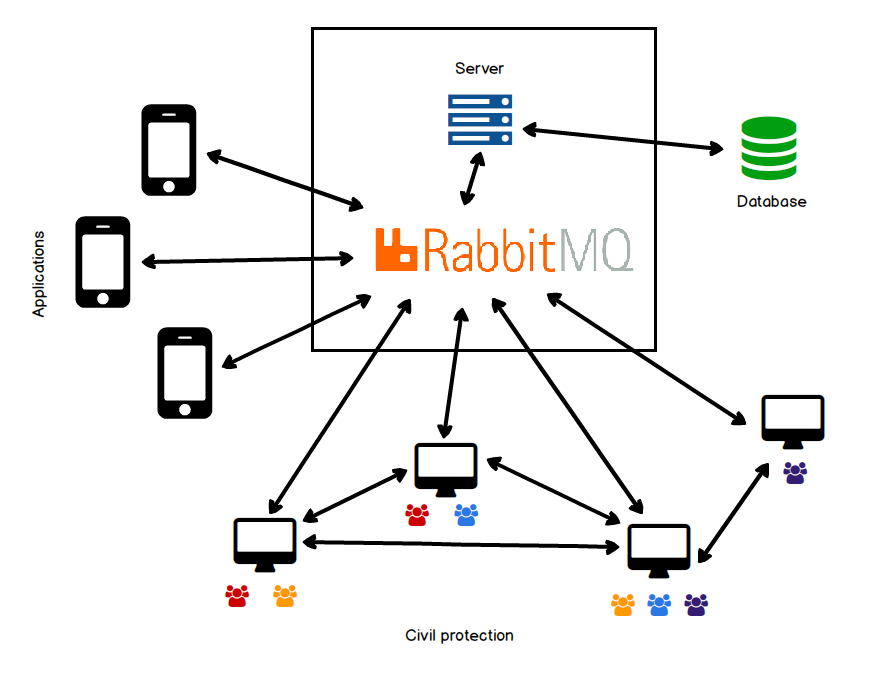
\includegraphics[width=\textwidth]{figures/BaseArchitecture.png}
\caption{System Architecture}
\label{fig:ArchDesign}
\end{figure}

\section{Patterns}

\subsection{Model-View-Controller}
As civil protection is a desktop application which consists of a relevant visual part, it has been handled using the Model-View-Controller pattern, that allows to decouple major components for efficient code reuse and parallel development.

As shown in figure \ref{fig:MVC}, MVC has been arranged with a major controller that communicates with four minor controllers, each one relative to a single view.

\begin{figure}[ht]
\centering
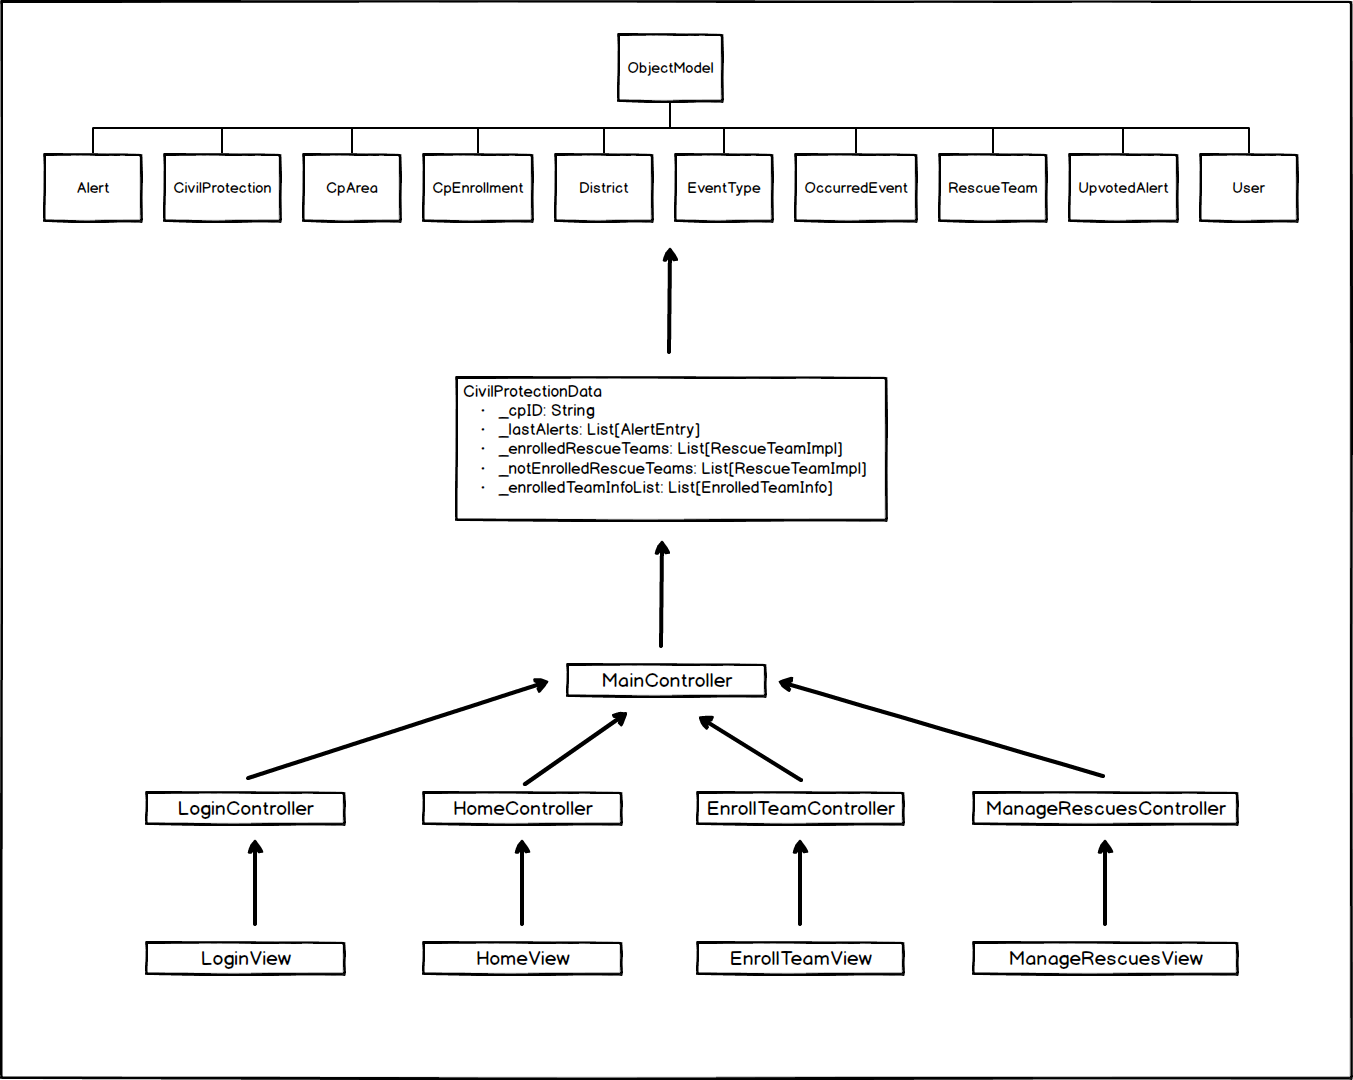
\includegraphics[width=\textwidth]{figures/MVC.png}
\caption{MVC}
\label{fig:MVC}
\end{figure}

%The MVC design pattern decouples these major components allowing for efficient code reuse and parallel development.
%https://en.wikipedia.org/wiki/Model%E2%80%93view%E2%80%93controller

%Con MVC si è gestito il modulo civilprotection in quanto è un applicativo desktop che comprende anche una parte rilevante di visualizzazione grafica.\\

%Disegno (controller grande + piccoli)\\
%Il design MVC è stato gestito come in figura X.\\
%Ognuna delle 4 view è associata ad un controller minore, il quale ha il riferimento ad un controller principale che ha il compito di interagire col modello.

\subsection{Data Access Object}
Data Access Object (DAO) is a commonly used pattern to persist domain objects into a database. The most common form of a DAO pattern is a class that contains CRUD methods for a particular domain entity type.
The pattern has these advantages:
\begin{itemize}
\item It separates the domain logic that use it from any particular persistence mechanism or APIs.
\item The interface methods signature are independent of the content of the implementation class. When you add a field to the Object of DAO, you don’t need to change the interface nor its callers.
\end{itemize}

A better pattern is Repository, it uses a metaphor of a Collection. This metaphor gives the pattern a tight contract and make it easier to understand.

In addition in this case, inheritance, abstract classes, and template methods are used to avoid duplicate code since all models need some common methods, this will be discussed in the next chapters.
So we have a GenericDAO, with the basic methods, from which all other DAOs extends.
In the following code segment is shown how a GenericDao is composed.

\lstinputlisting[label=lst:listato1]{code/DAO.java}

The \textit{insert} and \textit{delete} methods look identical to the methods of the simple DAO's, but the \textit{selectByIdentifier} method differs to the standard DAO’s \textit{findById} method by taking an ObjectModel object rather than the object identifier. 
Making this change you avoid to expose the type of ObjectModel identity to the interface.

In our case Repository pattern is realized with DAO.

\subsection{RabbitMQ Broker}
It was decided to adopt the Message-Oriented Middleware(MOM) RabbitMQ for the following reasons
\begin{itemize}
\item \textbf{Decoupling}: messages can be exchanged between system components which have been placed on the same or different network.
\item \textbf{Flexibility}: heterogeneous integration between technology stack and different types of clients is guaranteed by AMQP (Advanced Message Queuing Protocol implemented by RabbitMQ) whose main responsibility is the interoperability of the systems inside the messaging systems.
\item \textbf{Scalability}: system can scale horizontally easily by adding new Consumer.
\end{itemize}

A message producer produces messages and send them to the Message Broker which
routes messages to the right consumers. A message consumer await the upcoming messages, then process the information in them.

\subsubsection{Point-to-Point}
Point-to-Point communication has been used in communicating with the server where more clients can potentially send messages to a queue on which a server consumer of a specific service is waiting for messages.

When the server receives a message it is processed and the result can be 
\begin{itemize}
\item sent as a response 
\begin{figure}[ht]
\centering
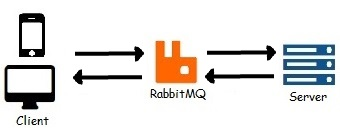
\includegraphics{figures/RPC.jpg}
\caption{Response}
\label{fig:RPC}
\end{figure}
\item forwarded to another client
\begin{figure}[ht]
\centering
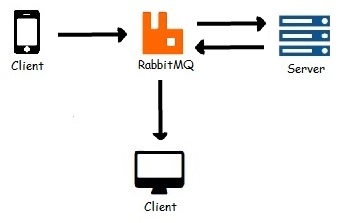
\includegraphics{figures/forward.jpg}
\caption{Forward}
\label{fig:forward}
\end{figure}
\end{itemize}

\subsubsection{Publish/Subscribe}
Publish/Subscribe communication has been used to send a message to multiple clients with consumer consuming on the same queue. 
Messages are not published directly to a queue, instead, the producer sends messages to an exchange.
An exchange is responsible for the routing of the messages to the different queues. 
The routing key is a message attribute added into the message header by the producer and it can be seen as an "address" that the exchange use to decide how to route the message. 
A message goes to the queue(s) whose binding key exactly matches the routing key of the message.
Subscribers needs to bind to the exchange in order to receive messages.
This is used when a civil protection notice all the other civil protecions about the availability of a specific rescue team.

\begin{figure}[ht]
\centering
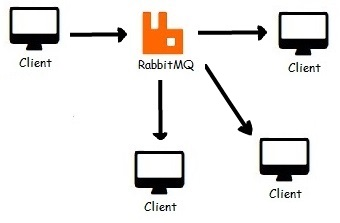
\includegraphics{figures/ps.jpg}
\caption{Publish-Subscribe}
\label{fig:PS}
\end{figure}

%(pattern architetturali usati, componenti del sistema distribuito, scelte tecnologiche cruciali ai fini architetturali -- corredato da pochi ma efficaci diagrammi)\\

%*) Ricordate che una scelta architetturale può ritenersi giustificata o meno (e dovremo capirlo) solo a fronte dei requirement che avete indicato\\

%*) L'architettura deve spiegare quali sono i sotto-componenti del sistema (da 3 a 10, diciamo), ognuno cosa fa, chi parla con chi e per dirsi cosa -- i diagrammi aiutano\\

%Disegnigno introduttivo è quello dell'Elisa


\chapter{Detail design}
%TODO
(pattern di progettazione, organizzazione del codice -- corredato da pochi ma efficaci diagrammi)\\
*) Il design di dettaglio "esplode" (dettaglia) l'architettura, ma viene concettualmente prima dell'implementazione, quindi non metteteci diagrammi ultra-dettagliati estratti dal codice, quelli vanno nella parte di implementazione

\section{Graphical User Interface Design}

Before the applications implementation, the graphical user interface design is an important stage. In this section, the applications mockups will be shown.

\subsection{Mobile App}

The graphical user interface for mobile application is designed to answer at all the functional requirements user side and to be user-friendly.

In the Figure \ref{fig:Mobilemockup}, the mockup realized for mobile application is shown. There are two main screens: one for the user not logged and one for the user logged.

The first main screen is designed to allow a user to login with his credentials and a new user to register.

The second main screen allows to a user logged to reach the screens to see all the last alarms in the district where the user is, to send a new alarm and to see and manage his profile.

\begin{figure}[ht]
\centering
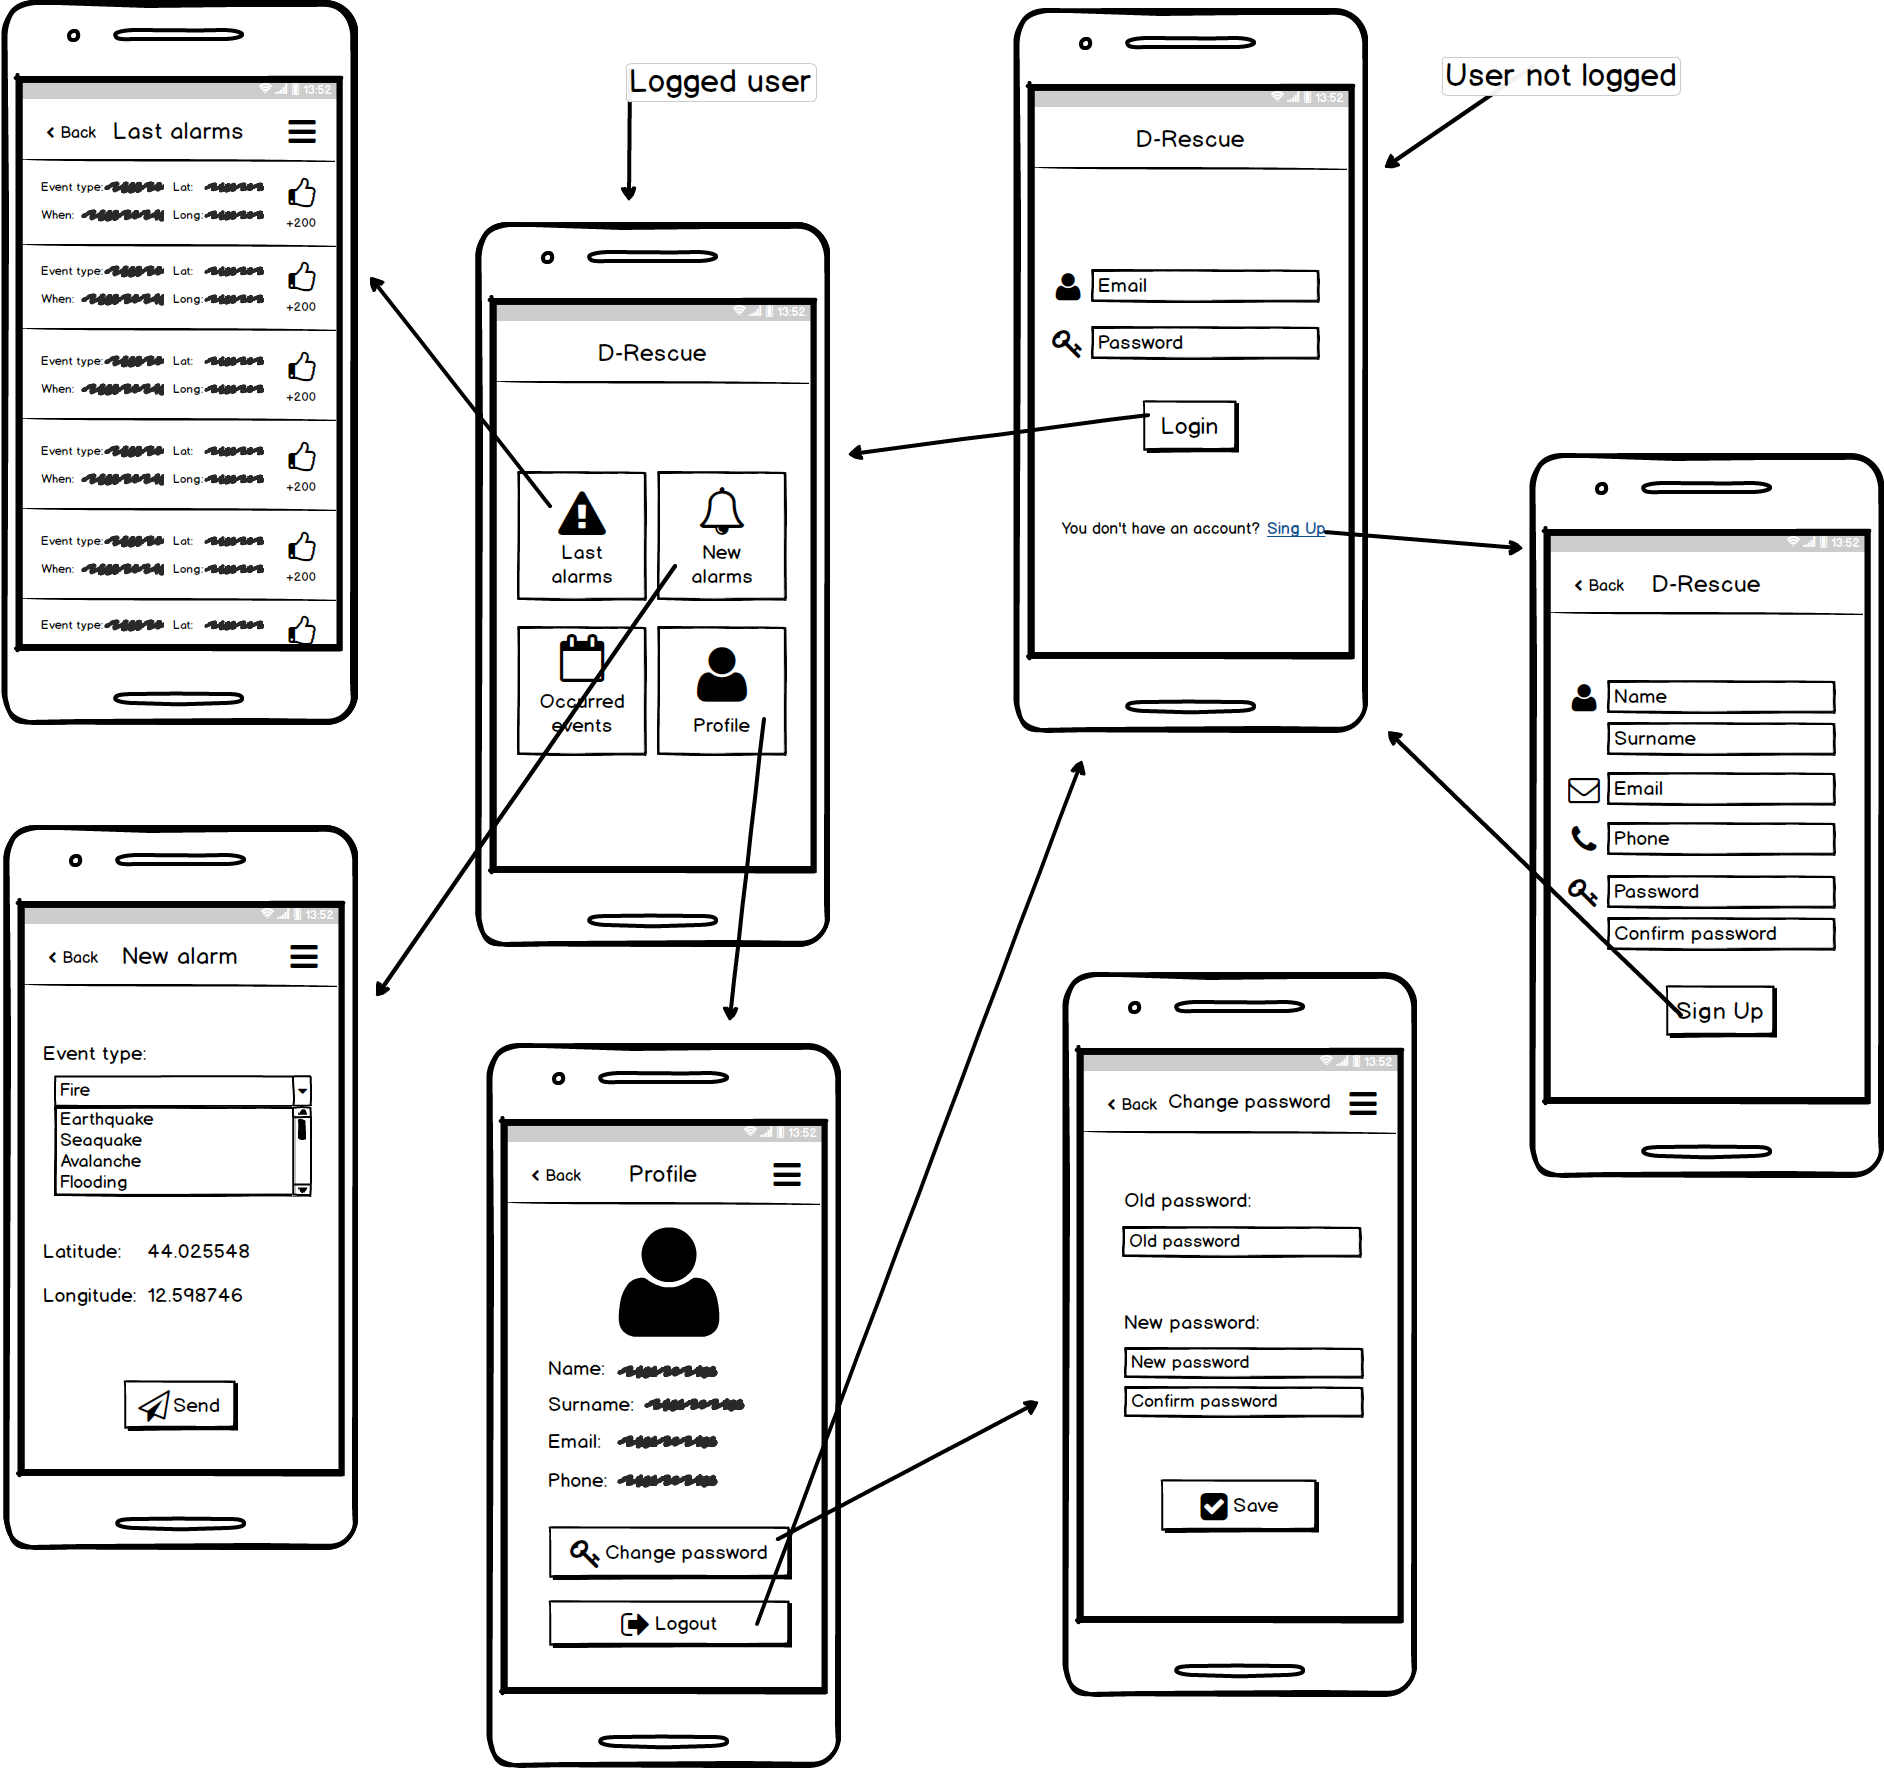
\includegraphics[width=\textwidth]{figures/mockupMobile.png}
\caption{Mobile user application mockups}
\label{fig:Mobilemockup}
\end{figure}

\subsection{Civil Protection}

\begin{figure}[ht]
\centering
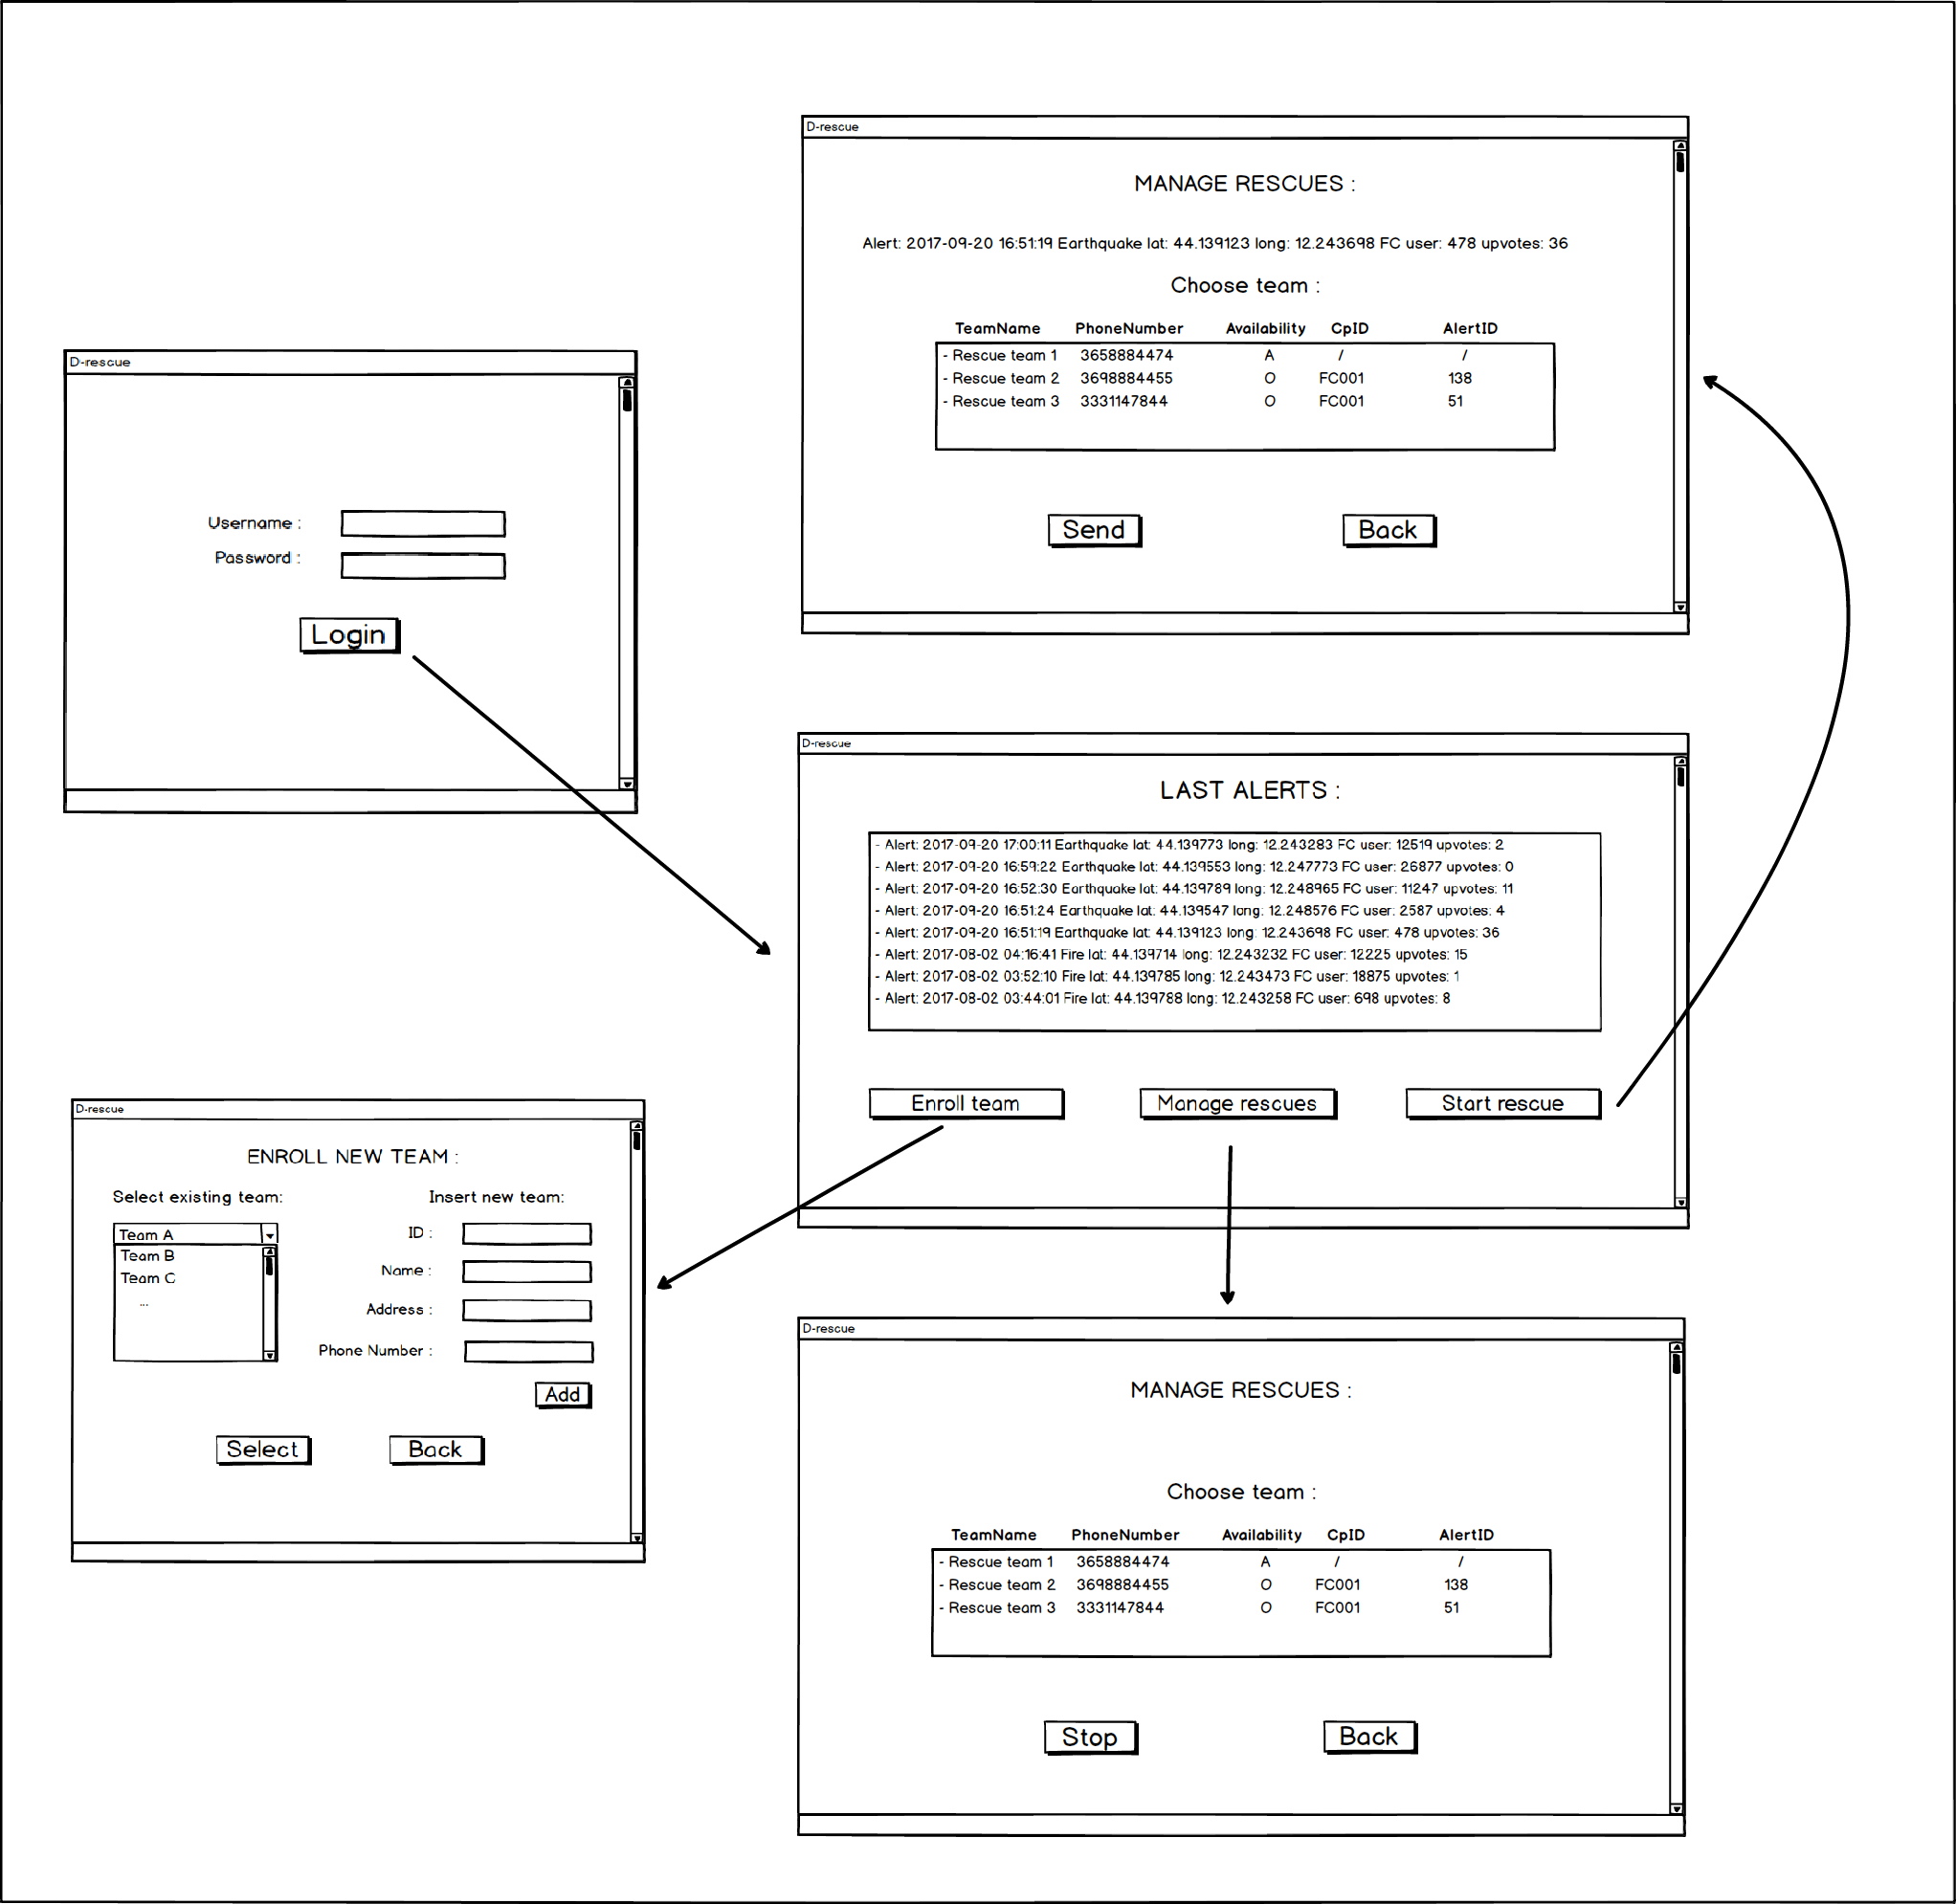
\includegraphics[width=\textwidth]{figures/CPmockup.png}
\caption{Civil protection mockups}
\label{fig:CPmockup}
\end{figure}

\section{Code organization}
The code is contained within the same project organized in modules.
\begin{itemize}
\item \textbf{civilprotection} module contains the civil protection application, which is organized according to the MVC pattern. 
\item \textbf{mobileuser} module contains the Android application 
\item \textbf{server} %contiene il codice dei servizi del server
\item \textbf{utils} module %TODO contiene il codice per eseguire le operazioni di geocoding e geodecoding ed i messaggi che le protezioni civili possono scambiare con il server 
\item \textbf{utils-java} module %contiene solo codice java, condiviso con gli altri moduli tra cui il model dell'interno progetto, le classi base per gestire la connessione con il RabbitMQ broker, la classe per serializzare e deserializzare i messaggi e le classi base per i messaggi ed i messaggi che l'applicazione mobile può scambiare con il server
\end{itemize}

\section{Server-DB}
AWS: deciso in remoto per evitare di avere copie duplicate e necessità di ricreare DB e server

MySQL: deciso per compatibilità con le varie componenti utilizzate (più conosciuto/più documentazione), gratuito.
Indecise con no sql poi scelto mysql perché db parecchio grande e per avere sicurezze di non incorrere in spese.

\section{Patterns}
\begin{itemize}
\item Builder: the builder pattern was used for model classes and those of messages that had more than 2-3 arguments at constructor.
\item Template Method: the template method pattern was used in handling server response in case of RPC and to group similar objects with common methods in accessing database.
\item Singleton: utilizzato per il coordinator %TODO
\item View-Holder: the view-holder pattern was used into Android adapter to store each of the component views inside the tag field of the Layout in order to access them without the need to look them up repeatedly. %TODO check!!!
\item Static factory: the static factory pattern has been used to create database connection. %TODO check
\item Factory pattern: the factory pattern has been used to retrieve the DAOs of database tables. %TODO check
\item Observer: used to manage the view update as a result of model changes. %TODO mettere una lista di observer observable?
\end{itemize}

\section{Communication messages}
As it was decided to use a Message-Oriented Middleware it was necessary to define a template for the many messages exchanged between system components. It is shown in figure \ref{fig:messageStruct}.

\begin{figure}[ht]
\centering
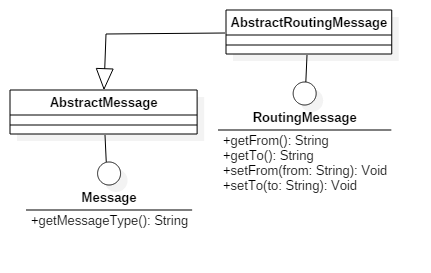
\includegraphics[scale=0.5]{figures/messages.png}
\caption{Base messages structure}
\label{fig:messageStruct}
\end{figure}

The tables below show the messages that are exchanged using point-to-point communication.

Mobile user - server communication:

\begin{center}
\begin{tabular}{ |p{4cm}|p{4cm}|p{4cm}|p{2cm}| } 
\hline
Service 			& Request message 	& Response message		& Type 	\\
\hline
Sign Up  			& SignUpMessage(name, surname,email,pass word,phoneNumber)		& SuccessfulMessage 	& RPC	\\ 
Login 				& LoginMessage(email, password) 	& ResponseLoginMessage (UserImpl,List$<$Event TypeImpl$>$)	& RPC	\\ 
Request profile 	& RequestProfileMessage (email)		& ProfileMessage(User Impl)	& RPC	\\ 
Change password		& ChangePasswordMess age(email,oldPassword, newPassword)	& SuccessfulMessage	& RPC	\\
Get alerts		& RequestAlertsMessage (latitude,longitude)	& AlertsMessage(List $<$AlertsImpl$>$)	& RPC	\\
New alert		& NewAlertMessage(user ID,eventType,latitude, longitude)	& no response but ForwardObjectMessage (List$<$String$>$,Object Model)	& p/s	\\
Upvote alert		& RequestUpvoteAlert Message(userID, alertID)	& no response but ForwardObjectMessage (List$<$String$>$,Object Model)	& p/s	\\
\hline
\end{tabular}
\end{center}

Civil protection - server communication:

\begin{center}
\begin{tabular}{ |p{4cm}|p{4cm}|p{4cm}|p{2cm}| } 
\hline
Service 			& Request message 	& Response message		& Type 	\\
\hline
Login	& CpLoginMessage(cpID, password)	& RescueTeamsMessage (List$<$RescueTeamImpl$>$) 	& RPC	\\ 
Get alerts CP	& RequestCpAlertsMes sage(cpID,password)	& AlertsMessage (List$<$AlertImpl$>$) 	& RPC	\\ 
Register team at CP		& EnrollRescueTeamMess age(rescueTeamID,cpID)	& SuccessfulMessage & RPC	\\ 
Get CP of rescue team 	& GetAssociatedCpMess age(rescueTeamID)		& CivilProtectionsMess age(List$<$CivilProtec tionImpl$>$)	& RPC	\\ 
New team	& NewRescueTeamMess age(rescueTeamID,name, password,latitude,lon gitude,phoneNumber)	& SuccessfulMessage	& RPC	\\
Get not enrolled rescue teams & GetRescueTeamsNot EnrolledMessage	& RescueTeamsMessage (List$<$RescueTeamImpl$>$)	& RPC	\\
\hline
\end{tabular}
\end{center}

The sequence diagrams in figure \ref{fig:seqRPC} and \ref{fig:seqForward} show two examples of successful scenarios respectivly for the response case and the forward one.

\begin{figure}[ht]
\centering
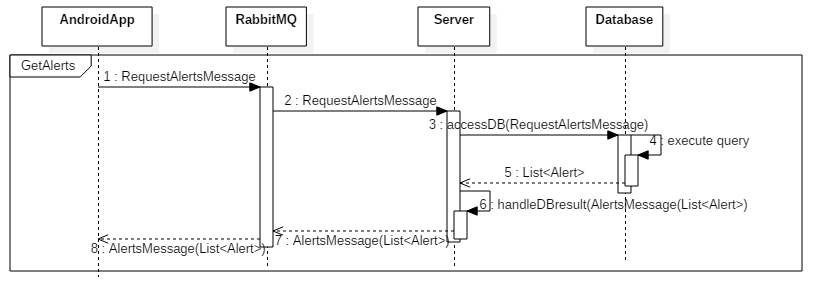
\includegraphics[scale=0.5]{figures/seqRPC.png}
\caption{Response Sequence Diagram}
\label{fig:seqRPC}
\end{figure}

\begin{figure}[ht]
\centering
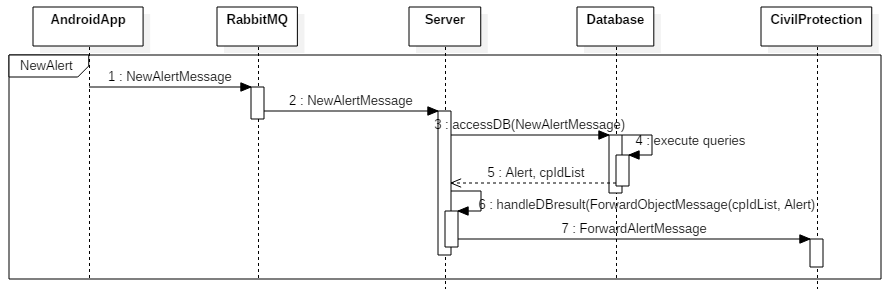
\includegraphics[scale=0.5]{figures/seqForward.png}
\caption{Forward Sequence Diagram}
\label{fig:seqForward}
\end{figure}

The table below shows the messages that are exchanged using publish/subscribe communication.

Civil protection - Civil protection communication:

\begin{center}
\begin{tabular}{ |p{4cm}|p{4cm}|p{4cm}|p{2cm}| } \hline
Service 			& Request message 	& Response message		& Type 	\\
\hline
Get Rescue Team Condition	& ReqRescueTeam ConditionMessage(RescueTeamID)	& ReplyRescueTeam ConditionMessage(RescueTeamID, RescueTeamCondition) 	& p/s	\\ 
Update Rescue Team Condition	&  ReplyRescueTeam ConditionMessage(RescueTeamID, RescueTeamCondition) 	& 	& p/s	\\ 
Coordination	&  ReqCoordinationMessa ge(RescueTeamID, reqTimestamp) 	& ReplyCoordinationMes
sage(RescueTeamID, rescueTeamCondition)	& p/s	\\
Coordination	&  ReplyCoordinationMessa ge(RescueTeamID, rescueTeamCondition) 	& 	& p/s	\\
\hline
\end{tabular}
\end{center}

\chapter{Implementation}

\section{Samantha Bandini}
In the DRescue project, Samantha Bandini contribution was mainly related to design and implementation of:
\begin{itemize}
\item Data Access Layer 
\item Handle Exception DB-Server in collaboration with Anna Giulia Leoni and Elisa Casadio
\item Handle MVC in civil protection in collaboration with Sofia Rosetti
\end{itemize}

\subsection{Data Access Layer}

Our application must access a database, so it needed some logic to handle database access. In order to keep the code clean and modular, the database access logic is isolated into a separate module, in our project is included in package\\ \texttt{server/src/main/java/it/unibo/drescue/database}. This package contains:\\

\subsubsection{DB connection classes}
%TODO fix packages
\texttt{DBConnection.java} and \texttt{DBConnectionImpl.java}: Respectively the interface and the class used to model the access method to DB and its tables.\\
It uses two static factory method instead of constructor, these methods, \\ \texttt{getRemoteConnection()} and \texttt{getLocalConnection()}, are static methods that returns an instance of the class with some specific settings for environment, like address, username and password used to connect to DB. One advantage of this pattern is that in this way it has name, in this case it was useful for specifying the criteria to choose the connection (local or remote).\\
As specified in previous chapters the DAO pattern was used for Data Access Layer. Since the DBConnectionImpl class is the one that keeps the general information about the database, information about DB tables are also maintained here, like its relative DAO. Here is maintained the enum with all table's name and the method \texttt{GenericDaoAbstract getDAO(final Table table)} which is a factory that returns the Dao relative to that table.\\

And the packages:\\

\subsubsection{DAO classes}
\texttt{dao}: It contains all DAO with their interfaces as specified in detailed design chapter.\\
%TODO fix: add link
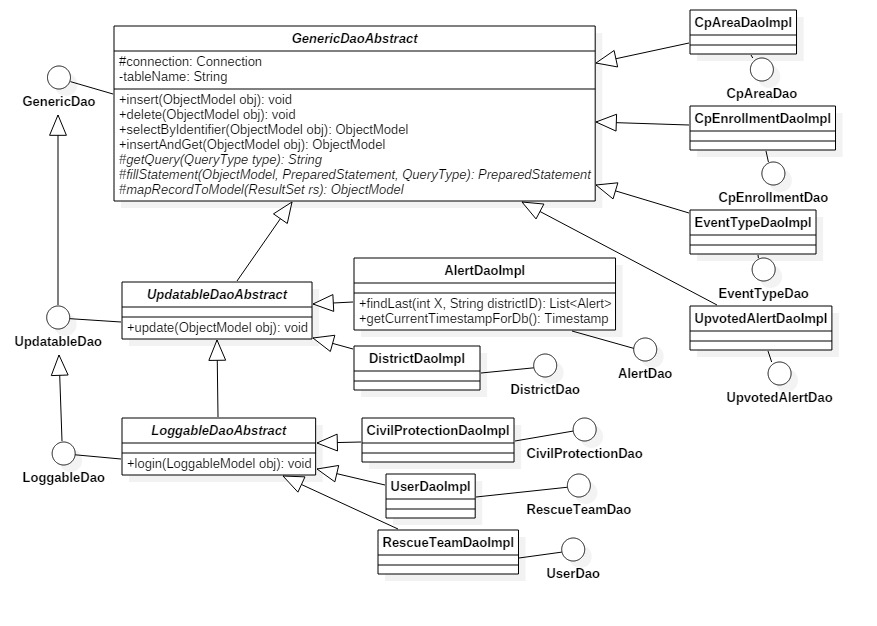
\includegraphics[width=\textwidth]{figures/ClassDiagram.jpg}
The DAOs are organized as specified in the partial class diagram above. Inheritance and template methods are used to group similar DAOs. The three main DAO's are GenericDao, LoggableDao, UpdatableDao. The GenericDao is the main class from which all others DAO extends, it contains the template methods insert, delete, selectByIdentifier, insertAndGet with abstract methods to be implemented in the classes that extend it.\\
The UpdatableDao contains the template method update, the LoggableDao contains the template method login and the abstract methods are:
\begin{itemize}
\item \texttt{String getQuery(final QueryType queryType)} Given a query type it returns the prepared query (a composed string) for this object
\item \texttt{PreparedStatement fillStatement(final ObjectModel objectModel, \\final PreparedStatement statement, final QueryType queryType)}: Given an object and a prepared statement it returns that prepared statement filled with the useful information to execute the specified query
\item \texttt{ObjectModel mapRecordToModel(ResultSet resultSet)} Get an object from a resultSet given, obtained from a select query by identifier
\end{itemize}

An example of a particular DAO is CpEnrollment, its method \\
\texttt{List<RescueTeam> findAllRescueTeamGivenACp(String cpID, boolean related)} has the parameter \textit{related} that is the criteria used to choose the query, since for the CpEnrollment we need both methods \texttt{findAllRescueTeamRelatedToACp} and \\
\texttt{findAllRescueTeamNotRelatedToACp}, with both returning a list of RescueTeam objects that differs only for the query. \\
Every DAO concrete class has been tested trying to isolate single pieces of the code. Following in broad terms the Test-Driven-Development, JUnit simple test classes have been written before each DAO class, and, in order to respect design principle also in test classes, these classes have been refactored. They can be found under the\\ \texttt{server/src/test/java/it/unibo/drescue/database} package.\\

%TODO check
\subsubsection{DB initialization classes}
\texttt{helper}: It contains the class DBInitializationStart used to initialize DB with static tables contents and some other data contained in externals file, to have something to start with.
The externals file are located in \textit{server/res}. The DBinitialization interface has a method used to insert into DB all objects listed in a json file, with a parameter \textit{table} that indicates the criteria, so in which table it has to be inserted, and the \textit{pathFile} that indicates the path where the file with objects is located.

To initialize the DB in this way, it was created in utils-java module, in package \texttt{src/main/java/it/unibo/drescue/database} a class \texttt{JsonFileUtils.java} with the generic method \texttt{<T> List<T> getListFromJsonFile(final String path, \\final Class<T[]> type)} that get a generic list of objects from a json file indicating the path of the file and the type of the class of the object to get.

\subsubsection{Travis configuration for mysql}
Tests that cover the database part must be run locally, so that they do not act on the remote database that is being used by the real application, but on a copy of this in local environment.
To do this, we had to prepare a .sql document to initialize all db tables and each of us, on a machine where SQL Server and SQL Workbench were installed, ran this file locally.
The problem came up when these tests had to be run in Travis. In addition to add the mysql service to the .travis.yml file, it was necessary to configure the credentials for Travis like in our local environment and also to create the DB with all tables. \\\
These rows has been added to .travis.yml file:\\
\texttt{before}\textunderscore\texttt{install:}\\
\texttt{- mysql -u root --password="" < travis.sql}
\\where travis.sql is a file .sql that contains all configuration specified above.

\section{Elisa Casadio}
The developed part mainly concerns the total or partial definition, design and development of the Android application and the server.

\subsection{Android application}
The code mentioned in this section is available in the \texttt{mobileuser} module.
\subsubsection{GPS}
GPS is a very important component within the application, as it is useful to indicate the exact location from which a user alert is sent and also to display all the alerts in the area where the user is located.

So, the application must have permissions to access the GPS, because the GPS is a sensitive data and it need to have the explicit consent of the user to be able to use it. Also, the device must have the GPS activated, because otherwise it would not be possible to understand where the user is and the latitude and longitude values could not be obtained.

The package \texttt{gps} contains an activity has been defined in which the required permissions and presence of the GPS provider are checked during creation and resume of activity. It also provides the latitude and longitude values, but if they aren't available it is setted a specific message. Using the \emph{observer} pattern, the activity is notified when the latitude and longitude values change or when the provider is disabled.

This activity is extended by all those activities that need to use the GPS, so that they can have the location values or check the provider.

\subsubsection{Layouts and Activities}
Four activities have been implemented with the relevant layouts to allow the user to send a new report, view the profile, change their password and the home page of application.

\begin{itemize}
\item \texttt{NewAlertActivity} in the package \texttt{alert} is the main feature that the application has, because it must allow the user to report a natural disaster. The class extends the GPS activity, because it needs to know the latitude and longitude values to show to the user and comunicate them to the server. In the layout, in addition to GPS values, it is given to user the possibility to select the type of natural disaster that occurs, by choosing between those in the database. The list of possible natural disasters is downloaded only whenever the user logs in so as not to slow down the operation and is saved between shared preferences of device.
\item \texttt{ProfileActivity} in the package \texttt{profile} shows the user data. The data are downloaded when the user logs in and they are saved in the shared preferences of the device. Each field is set by taking the value saved in the shared preferences that has a certain key. The keys that can be used are listed in the \texttt{PreferencesKey} enum in the package \texttt{utils}. From this activity is possible to reach the activity for change the profile password and do logout. The logout is very simple, just delete all the data saved in the shared preferences.
\item \texttt{ChangePasswordActivity} in the package \texttt{profile} allows the user to change his password. So, it is necessary to take the old and the new password, the user email and update his record on database. The layout shows three fields where the user can write. Each field must comply with two rules: the password must be at least 6 characters long and it must contain only alphanumeric characters.
\item \texttt{MainActivity} shows a RecyclerView where the CardView are arranged in a grid. Each CardView contains a title, an icon and a string with the class name that must start at the click of the CardView. The titles, the icons and the strings are listed in \texttt{arrays.xml} in \texttt{res} folder in the form of array. In order to handle the RecyclerView, it was need to use the \emph{Observer} pattern, the \emph{Adapter} pattern and the \emph{ViewHolder} pattern. Using the \emph{Observer} pattern, it was possible to notify when the user click on a specific CardView and to open the relative activity. The \emph{ViewHolder} pattern has allowed to set the correct fields of each CardView and the \emph{adapter} pattern has been the bridge between activity and the ViewHolder. \texttt{MainActivity}, during its creation or its resume, controls that the shared preferences are not empty. If this is not the case, it means that the user has logged out, so it need to go back to \texttt{SplashActivity} where the user can log in again.
\end{itemize}

\subsubsection{Connection between authentication and profile activities and server}
After performing all the layouts and basic activity operations, the connection between the activities and the server was added using the classes contained in the \texttt{connection} package.

The deployed connection is about authentication and profile activities. In all these cases, the type of communication is RPC, so all requests were made using \texttt{RabbitAsyncTask} class. The responses are \texttt{AbstractResponse}, so they were handled differently depending on what was needed to get. For more detailed explanation about \texttt{RabbitAsyncTask} and \texttt{AbstractResponse} see the dedicated section of developer Anna Giulia Leoni.

First, it was necessary to create a message to be sent to the server in order to forward the request, then check the presence of the Internet connection (both through mobile and Wi-Fi connecition). This check was essential because forwarding a request without connection could cause an application crash. Also, being necessary to recive a response from the server, it has entered a progress dialog that blocks the user's activity until the application receives any response from the server.

\begin{itemize}
\item \texttt{SignUpActivity} in package \texttt{authentication} was implemented by Anna Giulia Leoni and refactored by Elisa Casadio. The request message consists of all the data that the user has entered during the registration. The response message consists in a simple successful message, which confirm the database registration.
\item \texttt{LoginActivity} in package \texttt{authentication} has the request message assembled by the credentials of user. The response message consists in a message with the user data and a list of natural disaster. All this data are saved in shared preferences to use them in future in some requests or in the application. It has preferred to have all essential information at the user login, because it has avoided slowing down the user when displaying some views, such as profile or new alert.
\item \texttt{ChangePasswordActivity} in package \texttt{profile} has the request message assembled by the new and old password and the user email, the latter derived from shared preferences. The response message is a successful message, which confirm the update of password.
\end{itemize}

\subsubsection{Graphics}
To get a user-friendly application, the graphics were helpful. First, the basic colors that would have featured the application were choosen. Tones on green and yellow were chosen so that application could recall nature. Colors are listed within \texttt{colors.xml} so they can be used by all layouts. To have a minor repetition of the code, xml tags have been redefined within \texttt{styles.xml}, while \texttt{strings.xml} and \texttt{dimens.xml} have all the strings shown in the view and all the dimensions of the components used. Finally, the material icons were selected for use within the application.

\subsection{Server application}
In this section, the service exposed is located in \texttt{server} module in \texttt{connection} package.

\subsubsection{MobileuserService}
\texttt{MobileuserService} is a case classe used to implement useful operations to access database when requests are made on \texttt{MOBILEUSER\_QUEUE}. This queue takes all the requests concerning authentication and profile management.

The service decides what to do depending on the type of message. Possible message types accepted are:
\begin{itemize}
\item \texttt{SIGN\_UP\_MESSAGE} is the message sends when a user is registered into the mobile application. The user data are extracted from the request message and the user is inserted as a new record in the database. If the insert process is successful, \emph{SuccessfulMessage} is returned, otherwise, if an error occurs, it is captured. The email must be unique, so if it is duplicated, \emph{ErrorMessage} with a particular message is returned. This operations are implemented by developer Anna Giulia Leoni and refactored by developer Elisa Casadio.
\item \texttt{LOGIN\_MESSAGE} is the message sends when a user try to login into the mobile application. The user email and password are extracted from the request message and the user is searched into the user table of database. If the user is found, \emph{ResponseLoginMessage} is sent with all user data and a list of natural disaster, otherwise \emph{ErrorMessage} is sent, because email or password is wrong. If an error occurs, it is captured.
\item \texttt{CHANGE\_PASSWORD\_MESSAGE} is the message sends when a user wants change the password of his account. The user email, old password and new password are extracted from the request message. The user is searched into the user table of database, the old password send is compared with the real password and the user data are updated.
\item \texttt{REQUEST\_PROFILE\_MESSAGE} is usefull to get the profile of user. It is implemented for a future functionality. The user email is extracted from message and the user is searched into the user table. If the user is present, \emph{ProfileMessage} is sent with all the user data.
\end{itemize}

This service is tested with \texttt{scalatest} in class \texttt{MobileuserServiceTest} in the \texttt{connec-\\tion} package. For each type of message, the connection with a local instance of database is opened and operations of insert or update are run. Each test checks if the message type is the type expected. At the end, the fake user is deleted and the connection with database is closed.

\section{Martina Giovanelli}
In the DRescue project, Martina Giovanelli contribution was mainly related to design and implementation of communication between civil protections by way of the exchange of JSON messages and the management of rescue teams.
\subsection{Communication between civil protections}
Every civil protection maintain the condition of the rescue teams it has enrolled in in his local memory. 
When the civil protection receives a new alert it must communicate with each others in order to decide which rescue team send to solve the occured natural disaster reported by the users.\\
The rescue teams are shared among the different civil protections so, before select one, they must coordinate with others to recover the picked team status and update their local model.\\
The messages \texttt{ReplyRescueTeamConditionMessage} and\\ \texttt{ReqRescueTeamConditionMessage} inside \texttt{civilprotection} module are exchanged between the different civil protection respectively to request and send the condition of a particular rescue team.\\

We had to guarantee that the concurrent access of processes to a shared data (the rescue teams) is executed in mutually exclusive manner.
To satisfy this requirement we have dediced to use \textbf{ Ricart-Agrawala's algorithm}, a classical mission exclusion algorithm for distributive systems.\\

Communication between processes is based on the following assumptions:
\begin{itemize}
\item Processes communicate by reading and writing variables through the exchange of messages.
\item The delay of sending a message is unpredictable but finished.
\item The channel be reliable. A sent message is received correctly from its recipient. There are no duplications or spurious messages (received but never transmitted). 
\item The process do not fail. 
\end{itemize}

For the implementation of this algorithm two other message have been used:
\begin{itemize}
\item \texttt{ReqCoordinationMessage}
To request a rescue team, the civil protection sends a timestamped message to all processes.
\item \texttt{ReplyCoordinationMessage}
On receiving a request from any other civil protection, the process sends an OK message if either the process is not interested in entering in CS or if its own request has a higher timestamp value. Otherwise that message is kept in a pending queue.
\end{itemize}
Civil protection is granted the resource when it has requested the resource and it has received the OK message from every other
process in response to its request message.\\

The class \texttt{CoordinatorImpl} and the respective interface \texttt{Coordinator} inside the package \texttt{civilprotection/src/main/java/it/unibo/drescue/utils} represent a singleton used for the implementation of the above algorithm.\\
In particolar this class keeps the process status in relation to the critical section: \texttt{wanted}, \texttt{held} and \texttt{detached}.\\
The condition of the coordinator is equal to \texttt{wanted} when the civil protection wants to enter into critical section and updated the status of one  its rescue team. 
In this case the coordinator also maintains the timestamp of the request, the list ID of the civil protection from which the process expect an replay message and the critical section's name which corresponds exactly to the name of the rescue team.\\
The coordinator's condition is equal to \texttt{held} when the process is into critical section and \texttt{detached} when the civil protection isn't interested to occupied one team.\\
The coordinator keep the civil protection's condition for only one critical section.\\

\subsection{Rescues management}
Individual contribution in civil protection Model-View-Controller was mainly concerned the management of the rescue team into \texttt{ManageRescuesControllerImpl} class and the handle of the  messages received from other civil protection.\\
When the civil protection wants to occupied a rescue team it sends a  broadcast message to other civil protections that has enrolled in the same rescue team in order to received their local condition.
It waits until it received all the reply message or received a reply that inform it that the rescue team is already occupied.
In the first case the civil protection can occupied the rescue team in the other it must choose another team.\\
When civil protection wants to stopped the rescue team it update its local  condition from occupied to available and send a message to other civil protection to inform them about the updated team status.\\

\section{Anna Giulia Leoni}

The developed part mainly concerns the development of the Server application and the Android one, but also  a little part in the Civil Protection application.

\subsection{Server application}

All the code referred into this section is located into module \texttt{server/scala}.

\subsubsection{Service response, Service forward}
In order to handle the sending of a response and the forward of a message server side, \texttt{ServiceResponse} and \texttt{ServiceForward} traits were created in package \texttt{connection}. These traits extend \texttt{ServiceOperation} overriding and implementing in different ways \textit{handleDBresult}. 

Services that can handle both response and forward extends \texttt{ServiceResponseOr\\Forward} trait which extends both \texttt{ServiceResponse} and \texttt{ServiceForward}. This was possibile because Scala allows implementing functions in traits and multiple inheritance on traits. Basing on the content of the \textit{properties} parameter that came together with the message through RabbitMQ, it is discriminated if the message has to be forwarded or needs a reply and the appropriate \textit{super} method is called.
\\More specifically if the \textit{properties.getReplyTo} content is a valid string then represents the name of the queue to which send the response message returned from \textit{accessDB} method. Otherwise the result of the \textit{accessDB} method is a \texttt{FrowardObjectMessage} containing the ObjectModel to forward and the queues name to which forward it.
\\This behaviour is tested using ScalaTest inside \texttt{TestClientServerCommunication} class in \texttt{test} folder of package \texttt{connection}.
\\

\subsubsection{AlertsService}
Case class \texttt{AlertsService} in package \texttt{connection} extends \texttt{ServiceResponseOrForward} and manages messages requests related to alerts both from mobileuser and civil protection. More specifically these messages are shown in the detail design section.

In handling new alerts and upvotes messages is also necessary to retrieve the civil protections related to the zone from which the alert was sent to forward the alert or the upvote to the rights civil protections. Furthermore in handling new alerts and requests of alerts from mobile, methods of the Geocoding class were used to calculate the district to which register the new alert or to which get the alerts.

\subsection{Android application}

All the code referred into this section is located into module \texttt{mobileuser}.

\subsubsection{Layouts and Activities}
\texttt{ToolbarActivity} is extended by all the activities of the app. As the docs says the native ActionBar behaves differently depending on the Android version the device is using, we used Toolbar instead of ActionBar which has a more uniform behaviour.

Activities have been implemented with the related layouts to allow the user to sign up, login, get and upvote alerts.
\begin{itemize}
\item \texttt{SplashActivity} represents the splash screen of the app where the user can select to sign up or login
\item \texttt{SignUpActivity} and \texttt{LoginActivity} in package \texttt{authentication} represent respectivly the activity that contains the fields that the user must fill to sign up and login. Some checks are made on the validity of the email address and the match between password and confirm password at sign up.
\item \texttt{UpvoteAlertActivity} in package \texttt{alert} represents the activity that contains a list of existing alerts that the user can upvote to increase their reliability. It extends \texttt{GpsActivityImpl} because latitude and longitude of the user are needed to correctly download alerts of its district. \\
The alert list is presented within the app using Adapter and ListView. The \texttt{Alert Adapter} allows access to data and creates the corresponding view based on the layout provided for each alert of the given list. Inside the Adapter the ViewHolder pattern has been used to limit the number of calls to \textit{findViewbyId} method. This ways, this methods is invoked once for each item of the list passed at constructor and references to layout elements are stored in an \texttt{AlertViewHolder} instance associated with convertView with \textit{View.setTag} to be used for next items.
\end{itemize}

\subsubsection{Connection to server}
The package \texttt{connection} contains the classes used to communicate to the server and eventually parse the response.
\\To achieve this goal, Android AsynkTask were used. AsynkTask allows to perform background operations and publish results on the UI thread without having to manipulate threads and/or handlers. Within the \textit{doInBackground} method is contained the code to open the connection to the server, send the message and eventually waiting for a response.

More specifically two AsynkTask were created:
\begin{itemize}
 \item \texttt{RabbitAsyncTask} to perform RPC, returning a String result that represents the server response in json format. If the communication timeout is reached or in case of exception during the communication the result consists of an error. The received result is passed to an handler, represented by a class implementing the \texttt{RequestDelegate} interface, in our case \texttt{AbstractResponse} class, which deserializes it basing on message type and addresses it to the abstract methods \textit{onSuccessfulRequest} or \textit{onErrorRequest} implemented for each request to perform specific operations basing on it.
 \item \texttt{RabbitPublishAsyncTask} to send messages using the publish/subscribe paradigm, returning a boolean result that represents the sending outcome. The result is passed to an handler, represented by a class implementing the \texttt{PublisherDelegate} interface, which performs different operations basing on it.
\end{itemize}
The connection to the server was added into the activities of package \texttt{alert} using the above classes. Before sending the message to the server it is always checked that the device is connected to the netword and, if needed, if latitude and longitude values are correct. More specifically
\begin{itemize}
 \item in \texttt{NewAlertActivity} a \texttt{NewAlertMessage} containing the alert data is created, sent and the result of the sending is shown to the user.
 \item in \texttt{UpvoteAlertActivity} a \texttt{RequestUpvoteAlertMessage} containing the upvote data is created, sent and the result is shows as above; a \texttt{RequestAlertsMessage} containing user position is sent through RPC and on receiving the alert list of his district the adapter must be notified. If timeout is reached or an error occurr an error message is shown. 
\end{itemize}

\subsection{Civil Protection application}

All the code referred into this section is located into module \texttt{civilprotection}.

The developed part is strictly connected to request and response messages exchanged between civil protections in order to obtain information about the condition of their rescue teams.
\\These messages are \texttt{ReqRescueTeamConditionMessage} and \texttt{ReplyRescueTeamCondition\\Message}; their reception is handled inside \texttt{RescueTeamConsumer}. More specifically on receiving the first message the civil protection reply with the second one, setting as condition the one stored in \textit{EnrolledTeamInfo} local model for the specific rescue team; on receiving the second one the civil protection update its local model with the condition received.
A message to request enrolled rescue teams conditions is also sent at login and on enrolling a new team.

\section{Sofia Rosetti}
In the DRescue project, Sofia Rosetti contribution was mainly related to design and implementation of:

\begin{itemize}
\item Geocoding and reverse geocoding management
\item Model interfaces and classes
\item Civil protection views
\item Civil protection Model-View-Controller
\end{itemize}

\subsection{Geocoding and reverse geocoding management}
The geocoding and reverse geocoding service needed inside the project were designed and implemented using the Google Maps Geocoding API.

As Google explains, geocoding is the process of converting addresses (like a street address) into geographic coordinates (like latitude and longitude), while reverse geocoding is the process of converting geographic coordinates into a human-readable address.

As for the requirements of the project, it has been necessary to retrieve latitude and longitude coordinates giving a String corresponding to a generic address. This has been possible thanks to a \textbf{geocoding} request. The relative response consists in a JSON containing two root elements, ``status'' and ``results''. The ``results'' element contains an array of geocoded address and geometry information. From the geometry information it has been possible to retrieve the location, which returns latitude and longitude coordinates. 

Instead, \textbf{reverse geocoding} requests have been used to retrieve a district acronym (e.g. FC, RA, RN...) from latitude and longitude coordinates. The relative response contains a ``result'' element here too: instead of the geometry information, in this case we needed the ``address\_components'' information. 

It is composed of different elements like ``country'', ``root'' or ``street\_number'', but the interested one was ``\texttt{administrative\_area\_level\_2}'', which has a short name corresponding exactly to the district acronym we needed.

The \texttt{utils/src/main/java/it/unibo/drescue/geocoding} package contains geocoding interface, relative implementation class and exception class. Geocoding interface provides only two methods \emph{getDistrict()} and \emph{getLatLng()} that meet exactly the two requirements described above.

The \texttt{utils/src/test/java/it/unibo/drescue/geocoding} package contains a JUnit class test which verifies a proper operation.

\subsection{Model interfaces and classes}
In package \texttt{utils-java/src/main/java/it/unibo/drescue/model} there are all model interfaces and classes.

Every model entity represents one database table with all its attributes, so every interface provides methods to access and set the corresponding fields.

In the same package some other classes ending by ``Builder'' can be found. This because for class constructors with more than three fields the Builder pattern has been used.

Each model class has been tested trying to isolate single pieces of the code. For this purpose JUnit test classes have been written together with each model class. They can be found under the \texttt{utils-java/src/test/java/it/unibo/drescue/model} package.

\subsection{Civil protection views}
In order to mantain most of civil protection module implemented using the Scala language, views have been created by hand with \textbf{ScalaFX}. 

Views have been organized as following.

There is a \texttt{MainView} scala class, which represents the ``container'' class and has container elements, like \textit{stage} and \textit{scene}.
Then, four scala classes (\texttt{LoginGrid}, \texttt{HomeGrid}, \texttt{EnrollTeamGrid} and \texttt{ManageRescuesGrid}) represent the \textit{GridPane} which changes depending on the view to be displayed.
Every \textit{GridPane} is built with a row-column structure that allows to position elements and let them cover more than one row or one column.

The \texttt{MainView} provides a method to change the view that creates a new specific grid corresponding to one of the previous classes.

A \texttt{ViewConstants} object has been implemented too with the purpose of collecting all used constants and remove all magic numbers inside view classes.

\subsection{Civil protection Model-View-Controller}
Individual contribution in civil protection was firstly focused on the base application arrangement. The system has been designed following the Model-View-Controller pattern, therefore the views have to handle presentation and user interaction, the model handles the application logic and the controller coordinates model and views.

The civil protection controller is composed of five controller classes, one for each grid and a main controller. This because each grid only communicates with its relative controller, and then each controller can communicate with the main controller.

The grids' container class (\texttt{MainView}) has the reference of each controller in order to instanciate each grid with the proper controller. This has been implemented using the Builder pattern with named parameters.

Some buttons have been inserted to move among views. Every button has been provided of a mouse event able to catch the mouse click. So relative controller methods are called and all relative actions are performed in order to switch to the right view.

Part of the individual contribution was then oriented to implement two scala classes that belong to the civil protection local model.
The \texttt{AlertEntry} and \texttt{EnrolledTeamInfo} classes have been created to simplify insertion and values retrieval from the \textit{TableView} elements contained in the relative views. An \texttt{AlertEntry} element represents a table entry of the \texttt{HomeGrid}, because it's necessary to show the alert ID, the timestamp, latitude and longitude, the user and the district ID, the event name and the upvotes with a table representation. Similarly, the an \texttt{EnrollTeamInfo} element represents a table entry of the \texttt{ManageRescuesGrid}, because in this case it's necessary to show the team ID, name and phone number, if the team is available or not, the ID of the civil protection which occupied the team and the ID of the alert for which the team has been sent.

These two classes are also used in the \texttt{CivilProtectionData} class, which represents the model that every civil protection needs to mantain locally in order to get last alerts list and to manage rescue teams.

\section{Common parts}
%TODO Common part
Depending on the needs encountered during the implementation, messages were created by each of us with relative tests.

\subsection{Samantha Bandini - Sofia Rosetti}
All work has been carried out according to the pair programming technique.

\subsubsection{MVC package organization}

Civil protection application has been realized in order to focus on the management of data relative to the specific civil protection that is using the system.\\

Code has been organized as \texttt{civilprotection/src/main/scala/it/unibo/drescue/} package shows: 

\begin{itemize}
\item \texttt{controller} package: contains all controller classes.
\item \texttt{view} package: contains all views classes.
\item \texttt{localModel} package: contains classes relative to the logged civil protection local model. Generic model classes (which must be used from other modules too) can be found under \texttt{utils-java/src/main/java/it/unibo/drescue/model} package.
\end{itemize} 

Package localModel contains CivilProtectionData class, which represents the main local model to handle in each civil protection.


\subsubsection{Handle model in civil protection module using pattern Observer}

The views' real-time update has been set up with Observer pattern. Each model change produces a notification and the view is updated through an ObservableBuffer.

Observer pattern has been organized as following: the Observer trait is included in \texttt{civilprotection/src/main/scala/it/unibo/drescue/controller} package, as three minor controllers must implement it. This trait contains a \textit{onReceivingNotification()} method each observer class must implement in order to react to a notification.

In the same way, \texttt{civilprotection/src/main/scala/it/unibo/drescue/localModel} package contains the Observable trait, which is implemented by the CivilProtectionData class in order to notify a change. This trait has an object \textit{Observers} that represent an enumeration with which the right observer is notified. The \texttt{addObserver()} method is used to associate an observer to an observable object, while the \textit{notifyObserver()} method is used to notify the right observer through the enumeration.

\subsubsection{Handle communication from civil protection to server}
%TODO fix
La comunicazione client-server lato protezione civile è stata gestita per lo più dalle classi:\\

\texttt{RequestHandler.scala} la quale fa partire una future che ritorna un risultato, il quale è la risposta che deve essere interpretata dal controller in quanto è un messaggio codificato tramite formato JSON.


\texttt{AlertConsumer} è un consumer di RabbitMQ che rimane in attesa su una coda per ricevere i messaggi di ForwardAlertMessage e ForwardUpvotedAlertMessage; alla ricezione di questi messaggi provvede all'aggiornamento del model.\\

\subsection{Samantha Bandini - Elisa Casadio - Anna Giulia Leoni}
\subsubsection{Handle DB layer exeptions}
It was decided to handle database exception because to different exceptions corresponds different actions server side. All the database exceptions can be found in package \texttt{database/\\exceptions} of module \texttt{server/java}. More specifically
\begin{itemize}
\item a \texttt{DBConnectionException} is thrown if an error occurr while establishing or closing connection to database, or when asking to access a non-existing table.
\item a \texttt{DBQueryException} is thrown if an error occurr while executing a query.
\item a \texttt{DBDuplicatedRecordException} is thrown while inserting an object into database, when an equal object (with the same identifier) was found in database.
\item a \texttt{DBNotFoundRecordException} is thrown while searching an object into db, when an equal object (with the same identifier) was not found in database.
\end{itemize}
Sometimes when the last two occur, the error is notified to the client, otherwise it is only logged.

\subsection{Elisa Casadio - Anna Giulia Leoni}
\subsubsection{Server structure}
The code executed on server is located inside the \texttt{connection} package in \texttt{server} module.

\begin{itemize}
\item \texttt{ServerMain} represents the main class of the module, contains the code to setup the connection to RabbitMQ broker and runs all the services.
\item \texttt{Service} is a case class that represents a generic service. A new channel is created on the given connection and a new \texttt{ServerConsumer} is added to the channel to consume on the given queue.
\item \texttt{ServerConsumer} is a simple server-side consumer extending the default RabbitMQ consumer and overriding the \emph{handleDelivery} method called when consuming a message. Furthermore, a class implementing \texttt{ServerOperation} trait must be passed to the consumer in order to access database and handle potentially the returning result. In case of \emph{accessDB} method throw an exception, the error is logged, otherwise the result is handled. 
\item \texttt{ServiceOperation} is a trait modelling a general service to access database and handle the result. This trait is implemented by all classes that represent the specific services. The \emph{accessDB} method is where concreate access to database is using the Data Access Object.
\end{itemize}

\subsubsection{Server configuration}
Anna Giulia following AWS Guidelines setup a preconfigured instance with RabbitMQ called \emph{Bitnami}.

Elisa, however, configured the instance Linux machine. First, the Java 8 JDK and Scala 2.12.2 are installed to can run the application. A service is created so that the server application can always be active on the machine. The \texttt{drescue-server.sh} bash file, containing the script to create, start and stop the service on the machine, is added to \texttt{/etc/init.d/} folder. Inside the script, there is the command to execute the application jar.

\subsection{Martina Giovanelli - Anna Giulia Leoni}

\subsubsection{Setup the connection}
The package \texttt{connection} inside \texttt{utils-java} module contains the classes used to setup the communication through rabbitMQ used in every other module that needs to communicate with the server or other clients.
\\\texttt{RabbitMQConnectionImpl} class implements \texttt{RabbitMQConnection} interface and contains methods to setup, close and get the real TCP connection with the RabbitMQ broker by setting the host address, port, username and password. 
\\\texttt{RabbitMQImpl} class implements \texttt{RabbitMQ} interface and contains methods to setup, get and performs other operations related to the virtual connection (\textit{channel}) created on the TCP one like sending a message or adding a new consumer on the channel consuming on a specific queue.

\subsubsection{Message structure definition}
The package \texttt{communication/messages} inside \texttt{utils-java} module contains the template classes representing the messages exchanged within the entire system.
More specifically two type of messages have been created:
\begin{itemize}
\item \texttt{AbstractMessage} implementing \texttt{Message} interface which represents the message to be exchanged in client-server and server-client communication. 
\item \texttt{AbstractRoutingMessage} implementing \texttt{RoutingMessage} interface which represents the message to be exchanged in peer-to-peer communication to address the message to the right civil protections. 
\end{itemize}
This hierarchy is shown in the Detail Design section.

All the system components communicate through messages exchanged in JSON format. The chosen library for this aim is \textit{Gson}. \\
\texttt{GsonUtils} class is a simple wrapper of Gson that contains the method \textit{toGson} to serialize a generic Message into its equivalent JSON representation and the method \textit{fromGson} to deserialize the JSON String passed into a Message of the specified class.

%TODO chapter or section?
%\chapter{Testing}

\chapter{Retrospective}

%(descrizione finale dettagliata dell'andamento dello sviluppo, del backlog, delle iterazioni; commenti finali)\\

%*) Cercate di dare una idea di quanto pensate che i vostri test automatizzati coprano il codice e dove: è importante per stimare il potenziale impatto di una modifica al software\\


%Si noti che la retrospettiva è l'unica sezione che può citare aneddoti di cosa è successo in itinere, mentre le altre sezioni fotografano il risultato finale. Se gli studenti decideranno (come auspicato) di utilizzare un product backlog e/o dei backlog delle varie iterazioni/sprint, è opportuno che questi siano file testuali tenuti in versione in una cartella "process", così che sia ri-verificabile a posteriori la storia del progetto.

According to Agile metodology, we defined each Sprint at the end of the previous one and tasks have been divided among group members in base of preferences and previous knowledge.

Due to Martina Giovanelli's full-time work, she preferred to develop independently a part that didn't slow down general development process. Anyway, she took part of every Sprint closure together with other members.

During the first meetings we met face to face in order to discuss requirements and base architecture of the project, including some architectural pattern to adopt.
We set up all development environments, including the repository and the automatic build tools.

According to the requirements, we decided fundamental system parts to start with and other parts' priority.

We initially wanted to use a Platform-As-A-Service system regardless of the underlying infrastructure, in order to take advantage of the existing APIs. Because of this, we spent some time trying to learn the best way to use the Google App Engine platform.
Unfortunately, we encountered some problems. In Italy there is only the possibility to register a commercial account and not a private account. Moreover, the Flexible Environment we needed had only a Beta version of Java 8 and no Scala support.

For these reasons, we decided to switch on Amazon Web Services, which is an Infra-\\structure-As-A-Service. We set up two AWS instances, one for computation (\textit{Amazon Elastic Compute Cloud}) and one for the database (\textit{Amazon Relational Database Service}).

Initially, to test if the remote communication with AWS was working, we implemented the communication using sockets. We also tried to use Akka for communication between civil protections, but in the end we decided to use RabbitMQ in order to have the same communication type for both mobile and civil protection sides. This because RabbitMQ doesn't require to know each receiving address, but only the broker one and the queue to send requests on.

During development, most significant problems were related to:

\begin{itemize}
\item conflicts between Scala and Android, that brought to the creation of a separate module \texttt{utils-java}, containing only Java code;
\item \textit{AndroidILogger} IntelliJ bug, which disables all coding support and allows to find errors only during the build process. For this reason, we had to write only few lines of code before building the working module.
\end{itemize}

We also encountered difficulties in estimating each feature time. This brought to develop last project part (mainly related to the civil protection module) without technical excellence.

Finally, we discovered there is a problem with the RDS instance: sometimes responses are corrupted in spite of correct requests. This brings to the inability of accessing to the database data.
Development tests have been made with local server and local database, and nothing went wrong.

\section{Final judgement}

Although anyone had previously worked in a five people group, relationship and communication were good and each member was helpful with each other.

We are satisfied enough with the project result. In spite of some problems with the RDS instance, we reached a good result where communication brings to real-time updates of data and their relative transmission. It was important to reach this goal, because a possible future expansion may bring to a public benefit.

\section{Future developments}

Database and server have been already designed for possible future expansions, like :
\begin{itemize}
\item civil protections operating on common districts;
\item a session and an authentication token;
\item register real occurred events to keep events history;
\item a smart algorithm that knows which is the best rescue team to send for a rescue;
\item a smart algorithm that suggests when a rescue should be started basing on alerts, upvotes and districts population.
\end{itemize}

Other possible expansions are:

\begin{itemize}
\item showing a map with marks on alerts' location;
\item creation of a rescue team application to accept and notify the rescue end;
\item let the mobile user change his profile data;
\item encrypt passwords to improve system security.
\end{itemize}

\end{document} 